\documentclass{article}

\usepackage{graphicx}
\usepackage{tikz}
\usepackage{tikzsymbols}
\usetikzlibrary{calc,patterns,shapes.geometric}
\pagestyle{empty}
\usepackage[margin=0pt]{geometry}
\geometry{papersize={14in,12in}}

\def\centerarc[#1](#2)(#3:#4:#5){\draw[#1] ($(#2)+({#5*cos(#3)},{#5*sin(#3)})$) arc (#3:#4:#5);}

\begin{document}
	\begin{figure}
		\centering
		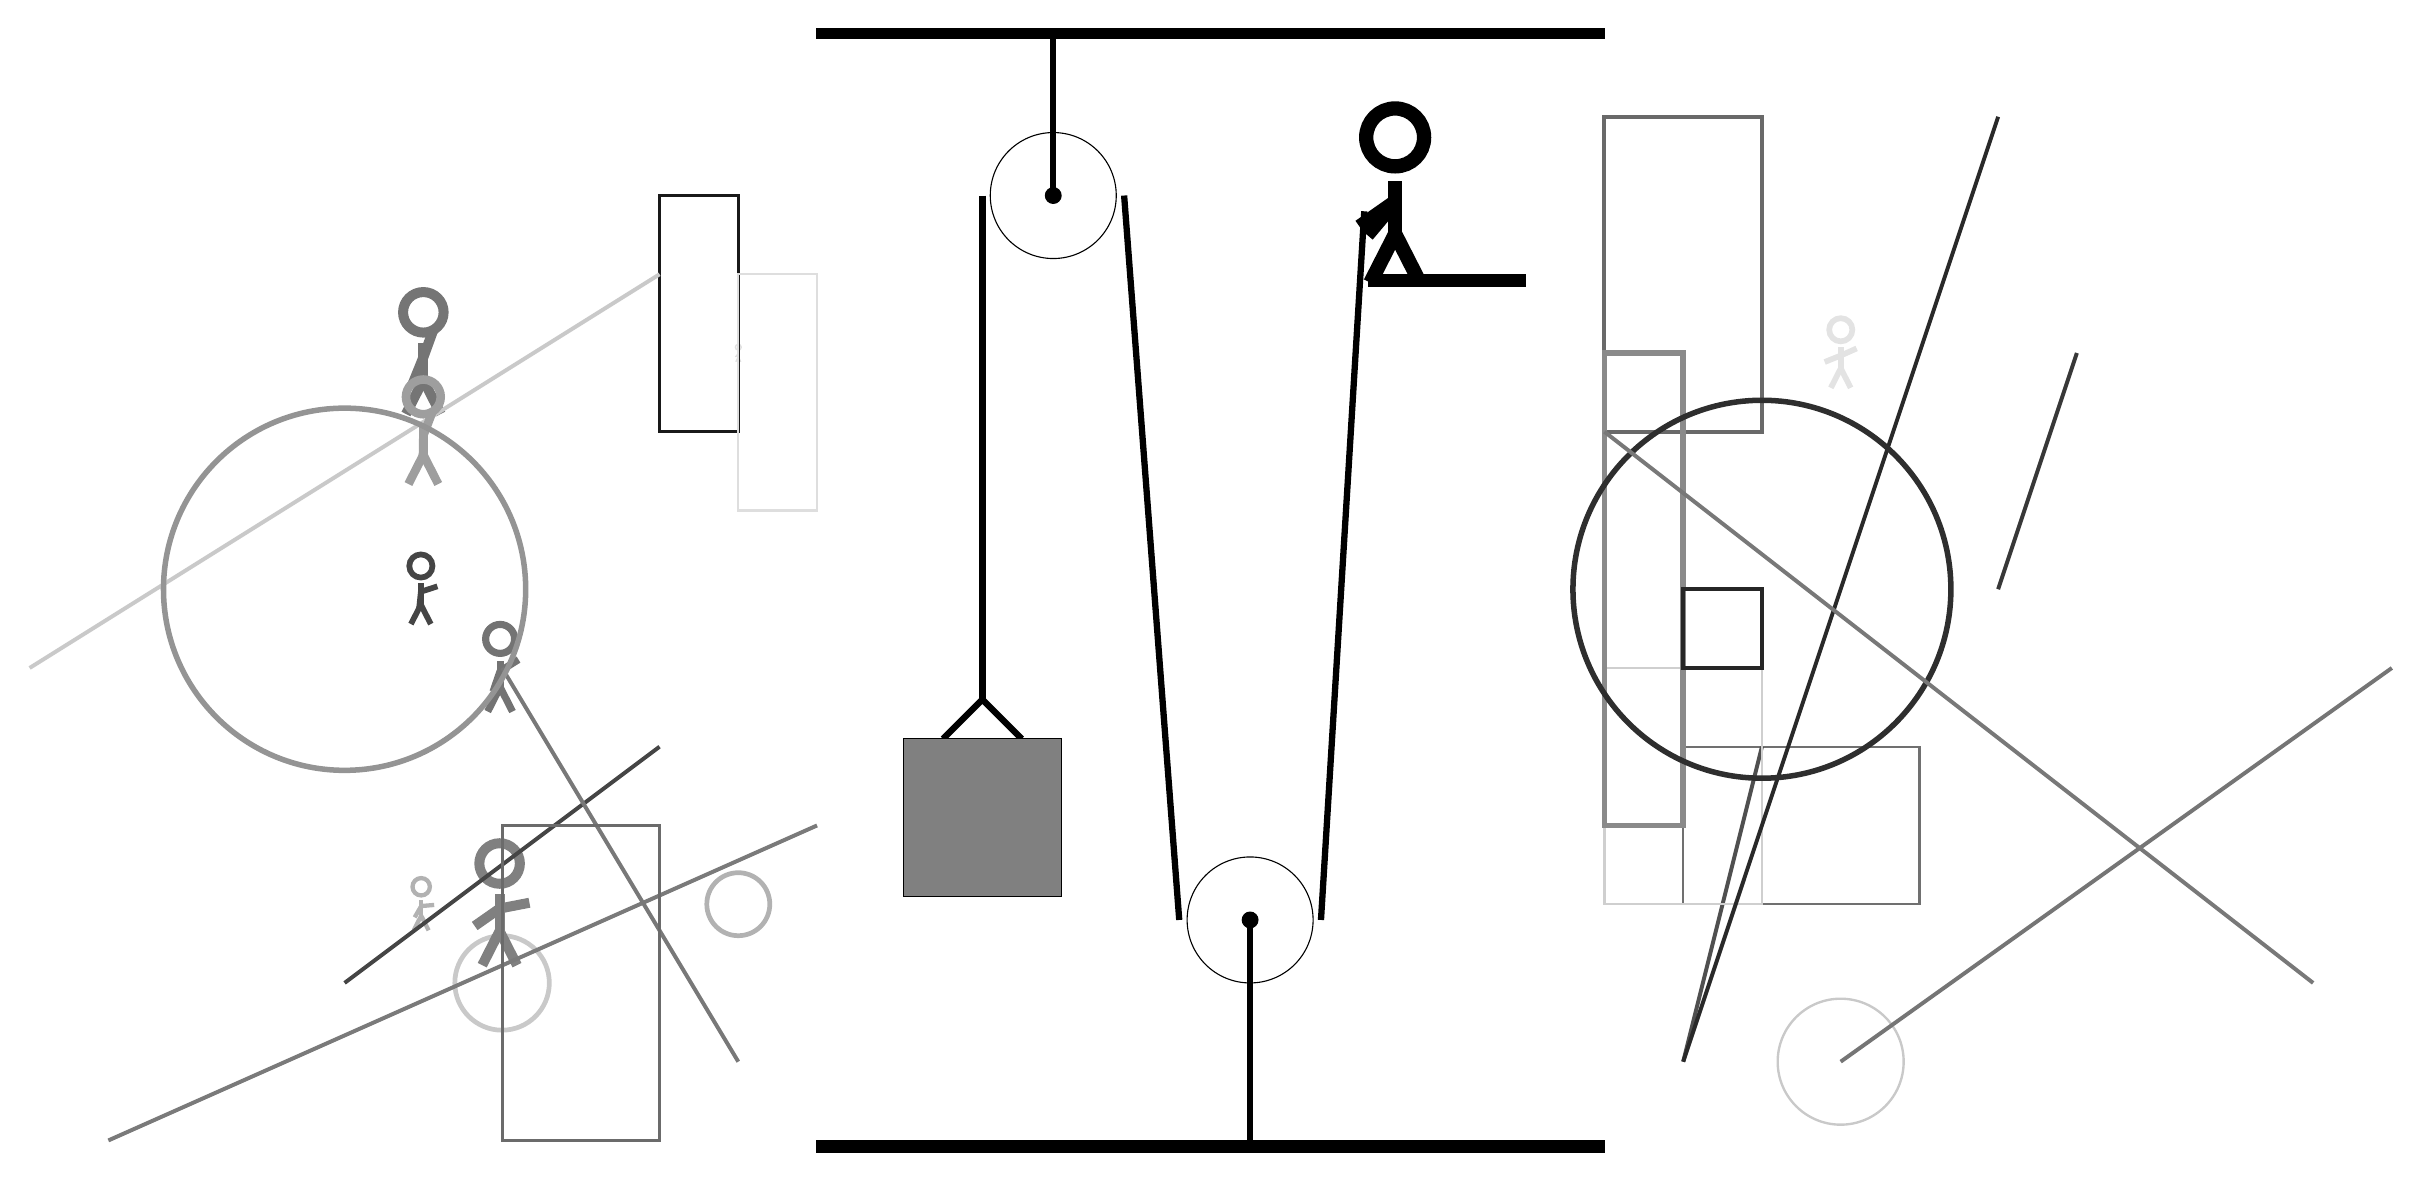
\begin{tikzpicture}
			%%%%% START %%%%%
			
			\draw[fill=black] (-2, 14) rectangle (8, 14.125);
			
			\draw (3.5, 2.8) circle (0.8);
			\draw[fill=black] (3.5, 2.8) circle (0.1);
			\draw[line width=0.8mm] (3.5, 2.8) -- (3.5, 0);
			
			\draw (1, 12) circle (0.8);
			\draw[fill=black] (1, 12) circle (0.1);
			\draw[line width=0.8mm] (1, 14) -- (1, 12);
			
			\draw[line width=0.8mm](-0.4, 5.1) --  (0.1, 5.6) -- (0.6, 5.1);
			\draw[fill=black!50] (-0.9, 5.1) rectangle (1.1, 3.1);
			
			\draw[line width=0.8mm](0.1, 12) -- (0.1, 5.6);
			\centerarc[line width=0.8mm](1, 12)(180:0:0.9)
			\draw[line width=0.8mm](1.9, 12) -- (2.6, 2.8);
			\centerarc[line width=0.8mm](3.5, 2.8)(180:360:0.9)
			\draw[line width=0.8mm](4.4, 2.8) -- (4.95, 11.8);
			
			\node at (5.3, 12) {\Strichmaxerl[10][35][-130]};
			\draw[fill=black] (5, 11) rectangle (7, 10.85);
			
			\draw[line width=0.5mm, color=black!59] (10, 9) rectangle (8, 13);
			
			\draw [line width=0.6mm, color=black!21](-6, 2) circle (0.6);
			\draw[line width=0.3mm, color=black!56] (9, 3) rectangle (12, 5);
			\node[line width=0.3mm, color=black!50] at (-6, 3) {\Strichmaxerl[7][35][11]};
			\draw[line width=0.5mm, color=black!52](-2, 4) -- (-11, 0);
			
			\draw [line width=0.3mm, color=black!21](11, 1) circle (0.8);
			
			\node[line width=0.2mm, color=black!73] at (-7, 7) {\Strichmaxerl[4][84][18]};
			\draw [line width=0.6mm, color=black!15](17, 3) circle (0.0);
			\node[line width=0.3mm, color=black!54] at (-7, 10) {\Strichmaxerl[7][68][70]};
			\node[line width=0.2mm, color=black!12] at (-3, 10) {\Strichmaxerl[1][50][74]};
			
			\node[line width=0.5mm, color=black!11] at (11, 10) {\Strichmaxerl[4][22][24]};
			
			\draw[line width=0.4mm, color=black!90] (-3, 12) rectangle (-4, 9);
			\node[line width=0.7mm, color=black!30] at (-7, 3) {\Strichmaxerl[3][60][5]};
			
			\draw[line width=0.5mm, color=black!54](11, 1) -- (18, 6);
			\draw[line width=0.5mm, color=black!69](9, 1) -- (10, 5);
			\draw[line width=0.3mm, color=black!19] (8, 3) rectangle (10, 6);
			\draw[line width=0.5mm, color=black!84](9, 1) -- (13, 13);
			
			\draw[line width=0.5mm, color=black!73](-4, 5) -- (-8, 2);
			\draw[line width=0.7mm, color=black!46] (9, 10) rectangle (8, 4);
			
			\draw[line width=0.5mm, color=black!21](-4, 11) -- (-12, 6);
			\draw[line width=0.5mm, color=black!78](13, 7) -- (14, 10);
			
			\draw [line width=0.7mm, color=black!82](10, 7) circle (2.4);
			
			\node[line width=0.2mm, color=black!55] at (-6, 6) {\Strichmaxerl[5][71][32]};
			\node[line width=0.5mm, color=black!38] at (-7, 9) {\Strichmaxerl[6][89][69]};
			\draw[line width=0.5mm, color=black!53](-3, 1) -- (-6, 6);
			
			\draw[line width=0.3mm, color=black!13] (-2, 8) rectangle (-3, 11);
			\draw [line width=0.6mm, color=black!30](-3, 3) circle (0.4);
			\draw[line width=0.5mm, color=black!53](8, 9) -- (17, 2);
			\draw[line width=0.4mm, color=black!58] (-4, 4) rectangle (-6, 0);
			\draw [line width=0.7mm, color=black!42](-8, 7) circle (2.3);
			\draw[line width=0.5mm, color=black!85] (10, 6) rectangle (9, 7);
			
			\draw[fill=black] (-2, 0) rectangle (8, -0.15);
			
			%%%%% END %%%%%
		\end{tikzpicture}
	\end{figure}	
\end{document}